\documentclass[11pt,a4paper]{article}
\usepackage[utf8]{inputenc}
\usepackage{amsmath}
\usepackage{amsfonts}
\usepackage{amssymb}
\usepackage{graphicx}
\usepackage{tikz}
\usepackage{multirow}
\usepackage{rotating}
\usepackage{cite}
\usetikzlibrary{positioning}

\author{Bastiaan Weijers \\ B.Weijers@students.uu.nl \\ 3256669 \and Colin Smits \\ C.Smits@uu.nl \\ 4075390}
\title{Evaluation of a Body Photo Browser\footnote{Word Count:3698}}
\renewcommand{\familydefault}{\sfdefault}
\begin{document}
\maketitle
\abstract{\noindent A computer vision systems recognising gestures in order to operate a photo browser is reviewed. The system evaluation focuses mainly on the accuracy of the system. We see that some gestures are confused, limiting the system's overall performance. The user evaluation is carried out by usability questionnaires. An overall evaluation is given using the PSSUQ, which shows that the system does not meet the standards set for a computer vision system. Parts of the system are evaluated using ASQ and SEQ, which show difference between tasks within the system. Linking both, we see that the way the system is running short of recognising gestures influences the user's perception of the system. }

\vspace{1cm}

\noindent \textbf{Keywords:} Computer vision, gesture recognition, system evaluation, user evaluation
 
\noindent\makebox[\linewidth]{\rule{\textwidth}{0.4pt}}

\section{Introduction}
The ease of using systems has become more important through the years. In order to check the usefulness, we need to evaluate the system. In this paper, we will discuss the usability of a body photo browser system, as will be defined later this section. The need for this is quite clear: the system is built for a user who wants a fluent experience, as well as a clear view of how to use the system. Taking this into consideration, we will discuss the system both from a system's perspective and the user's perspective.

The purpose of this evaluation is mainly to identify pitfalls in the system's accuracy, as well as recognising limiting factors for a satisfying user experience. We want to know what adaptations must be made to the current system in order to create an overall better performing system in terms of ease, satisfaction and accuracy.



In section 2, the system's reliability concerning robustness and accuracy will be discussed. For this, we will look at the accuracy of the system using a confusion matrix in order to get the system's precision and recall. After that, the usability of the system regarding ease of use and intuitiveness will be discussed in section 3 by the use of standard questionnaires (PSSUQ, ASQ and SEQ, see \ref{sub:userMeth}). Last but not least, a conclusion will be drawn based upon the evaluations in sections 2 and 3.

%INCLUDE research goals in introduction

\subsection{The system}
\label{sub:system}
The system is a body photo browser. Using the system, one is able to scroll through and rotate pictures in the Windows Photo Gallery software %insert source.
The following gestures are recognised by the system:

\begin{description}
\item[Swipe Left:] Using one hand (in view), going from right to left in the view. This will give the previous photo.
\item[Swipe Right:] Using one hand (in view), going from left to right in the view. This will give the next photo.
\item[Rotate left:] Using two hands (in view), going up with the right hand, and simultaneously going down with the left hand. This mimics the idea of rotating a picture counter clockwise.
\item[Rotate Right:] Using two hands (in view), going up with the left hand, and simultaneously going down with the right hand. This quite mimics the idea of rotating a picture clockwise.
\end{description}

The system works by recognising skin colour, then tracking the hands blobs through the screen, and depending on the total offset measured, a gesture might or might not be recognised and handled. 

\section{System Evaluation}
In this chapter we will discuss how the system evaluation was performed and what the results were of this evaluation.
 
\subsection{Methods and Environment}
To quantify the performance of the Body Motion program, we setup a test environment to measure how well the system can translate user interaction to concrete system actions. The test setup is contained in an ecologically sound environment, in this case a bedroom with closed curtains was used with as a primary light source three led bulbs lighting the room. There was a single participant used to create quantifying data, whereas the particular user was well introduced to the workings, capabilities and limitations of the system. 
5\\ The software was used with a YCrCb spectrum at [180 - 210] and a minimum delay of $70ms$ between actions, further settings were left at program-default.
\\ For each action performed in the video recording, a chart was updated with the value the system interpreted it to be. Possible predicted and actual actions were: Next, Previous, CW rotation, CCW rotation and Nothing. Whereas "Nothing" is represented as an idle action wherein nothing happens. It is worth noting that this particular action can only be actively observed on the actual outputs of the system, as predicting idle actions is not possible in our system.
%\par
%Furthermore, we go ahead and compare our data with data we gained as byproduct from the User Evaluation (Section 3). The comparison of these datasets will give an indication how representative the controlled environment for the system evaluation was.



\subsection{Results}
To achieve accurate and representing results, we have recorded a total of 159 actions that we will measure its interpretation by system off, this accounts to roughly 40 actions per possible move.  All actions are recorded in a total of two video's, this allows the system to run in a continuous mode, without having to reinitialize after every action. This continuous mode should yield results that are more ecologically sound as opposed to having system global variables reinitialized with every action.
\begin{table}
\begin{center}
\begin{tabular}{|c|c|c|c|c|c|c|}
\cline{3-7}
\multicolumn{2}{c|}{} & \multicolumn{5}{c|}{Predicted action} \\
\cline{3-7}
\multicolumn{2}{c|}{} & Next & Previous & CW & CCW & Nothing \\
\hline
\multirow{6}{*}{\begin{sideways} Actual action ~ \end{sideways}} & Next & 34 & 0 & 0 & 0 & 0 \\
\cline{2-7}
& Previous & 1 & 32 & 0 & 0 & 2 \\
\cline{2-7}
& CW & 0 & 0  & 22  & 4  & 6  \\
\cline{2-7}
& CCW  & 0  & 0  & 0  & 14 & 0  \\
\cline{2-7}
& Nothing & 2 & 5  & 16  & 21  & 0  \\
\hline
\end{tabular}
\end{center}
\caption{Testresults System Evaluation, $n=159$}
\label{table:systemeval}
\end{table}
\\ The evaluated output of a the actions will be tested against their expected outputs, the result of this can be found in Table~\ref{table:systemeval}. The data from the table shows the Predicted actions against the Actual actions delivered by the system for every possible action. From the table one can read how many predictions actually translated to correct behavior of the system, and how many did something unexpected.
\\ Table~\ref{table:systemeval} can be parsed to a so-called Confusion Matrix, which is depicted in Table~\ref{table:confusionmatrix}. This matrix is a further generalization and will help us in the question on how well our system performs. With a gesture controlled interface like the one tested, a preferred bias exists in having low false positives, possibly even in spite of an increased number of false negatives. From looking at the Confusion matrix we strongly suspect that we have satisfied this condition, but to confirm this we need to look at the Precision, Recall and Accuracy, shown in Table~\ref{table:systemevalvars}.
\par The system seems to perform mediocre if it comes down to the Accuracy and Recall, but it is quite $Precise$. 

\begin{table}[!h]
\centering
\begin{tabular}{lll}
\textbf{Accuracy}          & \textbf{Recall}            & \textbf{Precision}         \\
\multicolumn{1}{c}{67,5\%} & \multicolumn{1}{c}{69,9\%} & \multicolumn{1}{c}{95,3\%}
\end{tabular}
\caption{Accuracy, Precision and Recall of System Evaluation}
\label{table:systemevalvars}
\end{table}

\par
The data as presented can be further parsed into a confusion matrix which is shown in Table~\ref{table:confusionmatrix}.

\begin{table}[h]
\begin{center}
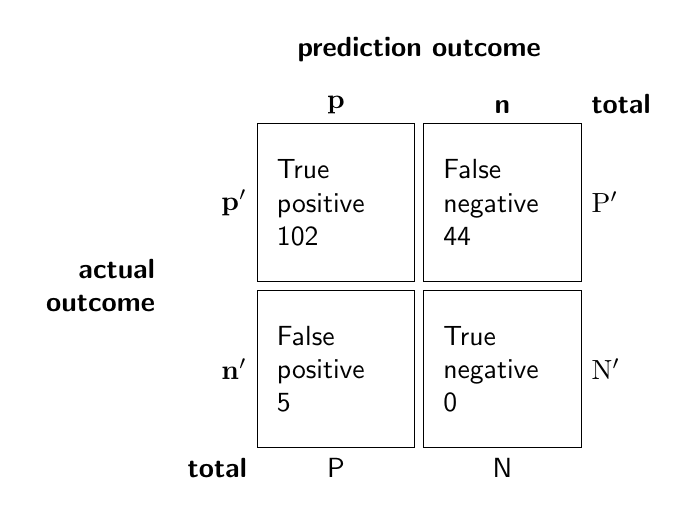
\begin{tikzpicture}[
box/.style={draw,rectangle,minimum size=2cm,text width=1.5cm,align=left}]
\matrix (conmat) [row sep=.1cm,column sep=.1cm] {
\node (tpos) [box,
    label=left:\( \mathbf{p'} \),
    label=above:\( \mathbf{p} \),
    ] {True \\ positive \\ 102};
&
\node (fneg) [box,
    label=above:\textbf{n},
    label=above right:\textbf{total},
    label=right:\( \mathrm{P}' \)] {False \\ negative \\ 44};
\\
\node (fpos) [box,
    label=left:\( \mathbf{n'} \),
    label=below left:\textbf{total},
    label=below:P] {False \\ positive \\ 5 };
&
\node (tneg) [box,
    label=right:\( \mathrm{N}' \),
    label=below:N] {True \\ negative \\ 0};
\\
};
\node [left=.05cm of conmat,text width=1.5cm,align=right] {\textbf{actual \\ outcome}};
\node [above=.05cm of conmat] {\textbf{prediction outcome}};

\end{tikzpicture}
\end{center}
\label{table:confusionmatrix}
\caption{Confusion Matrix}
\end{table}

\subsection{Discussion}
Having looked at and quantified obtained data, we now have a good idea of how well the system performs. One of the initial preference biases was the preference of a high Precision. Clearly, from look at Table~\ref{table:systemevalvars}, we see that the Precision is very high. However, the high precision comes at a price of having a mediocre Recall. Perhaps one might argue that the system was designed on forehand to prefer higher precision at the cost of yielding a lower recall, but the results don't lie and give a total of 67,5\% on the overall Accuracy.
\par From Table~\ref{table:confusionmatrix}, the confusion matrix, it seems that there exists a certain center of gravity if it comes down to where errors are produced. Namely CW/CCW rotations produce almost as much errors as successes. In this system evaluation an equal distribution over the actions was chosen, but perhaps there exists some difference in the usage of actions in the real world. So it could be that while Rotations generate a lot of errors, the actual usage of rotations by end-users might be low and thus resulting in a higher recall and accuracy.

\section{User Evaluation}
Now that we have had a look from a system point-of-view, we will now evaluate the system from a user perspective. First, the used methodology will be discussed. After that, the results and discussion will follow.

\subsection{Methods and Environment}
\label{sub:userMeth}
In our user evaluation, we want to see whether our system is intuitive and easy to use. In order to do that, we need to have a number of people testing our system. First of all, we need to define the environment in which we will be testing. Using the notion of ecological validity, which states that the surroundings in which the research takes place must resemble a real-world setting\cite{brewer2000research}, the tests will take place in normal rooms in terms of for example lighting and background. A laboratory would not be suitable as the user will react differently. The tests are then carried out as follows. 

First of all, we ask the user to take a look at the system. We have defined four different gestures, and for each of the different options, we ask the user what would be his first opinion on how to perform the task. The user will give his own gesture which he would use in order to perform the action. That way, we can compare the thoughts of users to our own throughts on the used gestures. After that, we set up 10 scenarios, as shown in Table \ref{tab:scen}. The first four scenarios contain each of the different gestures in order to make the user comfortable with the system. After that, we start combining the gestures so that the user should be thinking about what gestures he must use in which order. Finally, we do not specify the gestures any more, but we describe the task by specifying pictures the user must recognise. In this way, we can test whether the user can perform the right actions while still thinking of what to do. The last part mainly shows how intuitive and easy our system can be used, as the user will be distracted from the gestures. 

\begin{table}
\begin{center}
\begin{tabular}{r|l}
\textbf{Scenario} & \textbf{Task} \\
\hline
1 & Navigate to the next photo \\ 
2 & Navigate to the previous photo \\
3 & Rotate the photo clockwise \\
4 & Rotate the photo counter-clockwise \\
5 & Navigate to the second next photo (twice to the next)\\ 
6 & Rotate the previous photo clockwise \\
7 & Rotate the photo and put it back up \\
8 & Navigate to the photo containing [something] \\
9 & Put the current (rotated) photo back up \\
10 & Navigate to the rotated photo and put it back up \\
\end{tabular}
\end{center}
\caption{\textit{Specified scenarios in the user tests}}
\label{tab:scen}
\end{table}



Secondly, in order to get measurements, we set up a questionnaire. According to Sauro and Lewis \cite{sauro2012quantifying}, and Tullis and Albert \cite{albert2013measuring}, there are different standardized questionnaires. For our system, we want to know whether the user is satisfied with the system as a whole. As defined by Sauro and Lewis, the PSSUQ (Post-study System Usability Questionnaire) is "designed to access users' perceived satisfaction with computer system applications" \cite{sauro2012quantifying}. Looking at our goal, we think this questionnaire fits our research. Therefore, we incorporated this questionnaire at the end of the test, after all the scenarios have been completed. We chose the PSSUQ over the SUS (System Usablity Scale), which can also be used as a measure of the usability of a system, due to an increased reliability \cite{sauro2012quantifying}.

In addition, we thought that the user should be able to tell us what he perceived during each scenario. For that, we set up a combination of the ASQ (After Scenario Questionnaire) and the SEQ (Single Ease Question). The ASQ was developed by Lewis in order to describe the user's satisfaction with completing a certain task \cite{sauro2012quantifying}\cite{lewis1995ibm}. This can be perfectly used for our research goal. Moreover, the ASQ is linked to the PSSUQ, and also describes the user's satisfaction with a system, in this case a certain task. Furthermore, as the name suggests, the SEQ is used to describe a user's view on the ease of completing a task. The combination is used to get more reliable results.

\subsection{Results}
To start off, we look at the user's thoughts on the gestures to be used. In Table \ref{tab:compGes}, we show the percentage of user's defining a certain gesture for an action. We can see that for the navigation actions, the users differ in view, whereas for rotations, all the users say the same.
\renewcommand{\arraystretch}{1.5}
\begin{table}[h!]
\begin{center}
\begin{tabular}{l || l | c}
\textbf{Action} & \textbf{ Users opinions} & \% \\
\hline
\multirow{2}{*}{Next photo} & Hand left to right & 43 \\
 & \textbf{Hand right to left }& \textbf{57} \\
\hline
\multirow{2}{*}{Previous photo} & \textbf{Hand left to right} & \textbf{57}\\
& Hand right to left & 43\\
\hline
\multirow{2}{*}{Rotate left} & Rotate hands in circle counter-clockwise & 100 \\
& \textbf{Left hand down, right hand up} & \textbf{0} \\
\hline
\multirow{2}{*}{Rotate Right} & Rotate hands in circle clockwise & 100 \\
& \textbf{Left hand up, right hand down} & \textbf{0}
\end{tabular}
\end{center}
\caption{\textit{Comparison of the implemented gestures (in \textbf{bold}) with the user's opinions on the gestures to be used. $ n = 7$}}
\label{tab:compGes}
\end{table}


After that, we need to examine the results from the questionnaires. We will start by analysing the scenario questionnaires, the SEQ and ASQ.
Firstly, the SEQ results are shown in Table \ref{tab:seq}. On first glance, we can see that for the scenarios containing only navigating to photos, the overall score is low ( $<$ 3), as opposed to those only containing rotations ( $>$4). Furthermore, the more complicated tasks show a broad confidence interval, meaning that there is much variation between users as far as ease of use is concerned. \\

\renewcommand{\arraystretch}{1.0}
\begin{table}[h!]
\begin{center}
\begin{tabular}{c  l || c || c | c}
\textbf{Scenario} & \textbf{Description} & 
\textbf{Lower} &
\textbf{Mean} &
\textbf{Upper} \\
\hline
1 & Navigate to the next photo & 0.93 & 2.43 & 3.93 \\
2 & Navigate to the previous photo & 0.93 & 2.43 & 3.93 \\
3 & Rotate the photo clockwise & 1.84 & 3.43 & 5.02 \\
4 & Rotate the photo counter-clockwise  & 1.84 & 3.43 & 5.02 \\
5 & Navigate to the second next photo & 1.59 & 2.29 & 2.98 \\
6 & Rotate the previous photo clockwise & 1.55 & 2.71 & 3.87 \\
7 & Rotate the photo and put it back up & 1.55 & 2.71 & 3.87\\
8 & Navigate to the photo containing [something]& 1.39 & 2.57 & 3.75\\
9 & Put the current (rotated) photo back up  & 1.03 & 2.42 & 3.83\\
10 & Navigate to the rotated photo and put it back up & 1.41 & 2.28 & 3.17\\
\end{tabular}
\end{center}
\caption{\textit{Results of the SEQ, showing the mean and 95\% confidence intervals for each of the scenarios. $n=7$}}
\label{tab:seq}
\end{table}

\begin{table}[h]
\begin{center}
\begin{tabular}{l | llllllllll}
            & \textbf{1} & \textbf{2} & \textbf{3} & \textbf{4} & \textbf{5} & \textbf{6} & \textbf{7} & \textbf{8} & \textbf{9} & \textbf{10} \\
\hline
\textbf{1}  & 1.00       & -          & -          & -          & -          & -          & -          & -          & -          & -           \\
\textbf{2}  & 0.69        & 1.00       & -          & -          & -          & -          & -          & -          & -          & -           \\
\textbf{3}  & 0.76       & 1.00       & 1.00       & -          & -          & -          & -          & -          & -          & -           \\
\textbf{4}  & -0.97      & -0.5       & -0.58      & 1.00       & -          & -          & -          & -          & -          & -           \\
\textbf{5}  & 0.76       & 1.00       & 1.00       & -0.58      & 1.00       & -          & -          & -          & -          & -           \\
\textbf{6}  & 0.69       & 1.00       & 1.00       & -0.50      & 1.00       & 1.00       & -          & -          & -          & -           \\
\textbf{7}  & 0.33       & 0.91       & 0.87       & -0.09      & 0.87       & 0.91       & 1.00       & -          & -          & -           \\
\textbf{8}  & 1.00       & 0.69       & 0.76       & -0.97      & 0.76       & 0.69       & 0.33       & 1.00       & -          & -           \\
\textbf{9}  & 0.50       & -0.28      & -0.19      & -0.69      & -0.19      & -0.28      & -0.28      & 0.50       & 1.00       &             \\
\textbf{10} & 0.50       & 0.97       & 0.95       & -0.28      & 0.94       & 0.97       & 0.97       & 0.50       & -0.50      & 1.00       
\end{tabular}
\caption{\textit{Results of the ASQ, showing the correlation of overall usability between scenarios, $n=7$}}
\label{tab:ASQ}
\end{center}
\end{table}

The results from the ASQ are depicted in Table \ref{tab:ASQ}. Each cell represents the correlation of the scenarios as obtained after doing a factor analysis on the data gotten. Striking is the fact that scenarios 2, 3, 5 and 6 are tightly correlated in terms of ease. However, in comparison with scenario 1, which is opposite of scenario 2, these scenarios do not have a strong correlation.\\

Now we need to study the user's satisfaction overall. In Table \ref{tab:pssuq}, the results from the PSSUQ questionnaire are shown. For each question, the mean of the scores is shown as well as the values for the 95\% confidence intervals. At the bottom, the averages per group of questions is shown, in compliance with the grouping of questions according to Sauro and Lewis \cite{sauro2012quantifying}.

\begin{table}[t!]
\begin{center}
\begin{tabular}{c || c || c | c}
\textbf{Question} &
\textbf{Lower} &
\textbf{Mean} &
\textbf{Upper} \\
\hline
1 & 2.08 & 2.57 & 3.06 \\
2 & 1.70 & 2.43 & 3.15 \\
3 & 2.26 & 2.71 & 3.17\\
4 & 1.87 & 2.86 & 3.85 \\
5 & 0.93 & 2.00 & 3.07 \\
6 & 2.84 & 3.57 & 4.30 \\
7 & 4.73 & 5.86 & 6.98\\
8 & 1.90 & 3.14 & 4.39\\
9  & 2.31 & 4.29 & 6.26\\
10 & 2.31 & 4.00 & 5.69\\
11 & 1.59 & 3.43 & 5.27\\
12 & 3.40 & 4.86 & 6.31\\
13 & 1.44 & 2.71 & 3.99\\
14 & 2.22 & 2.86 & 3.99\\
15 & 2.25 & 3.43 & 4.61\\
16 & 2.03 & 2.86 & 3.69 \\
\hline 
\hline
Avg. 1-6 & 1.95 & 2.69 & 3.43 \\
Avg. 7-12 & 2.71 & 4.26 & 5.82 \\
Avg. 13-15  & 1.97 & 3.00  & 4.03 \\
Avg. 1-16  & 2.24 & 3.35 &  4.46 \\
\end{tabular} 
\caption{PSSUQ results showing the mean for each question compared to the 95\% confidence intervals. $n=7$}
\label{tab:pssuq}
\end{center}
\end{table}

\pagebreak

\subsection{Discussion}
From the results obtained for the user's opinion on the gestures, we can conclude that the navigation is something that matters from person to person. The intention of the implemented gesture was to simulate a swipe on, for example, a tablet. To go to the next photo, one must then swipe from right to left, seemingly pushing the photo roll to the left. However, users perceive that it could also be seen as the direction to where one wants to go. In this case, the meaning of a swipe to the left is that the photo to the left should be shown, thus the previous. This is something that has to be worked out further. 

Another striking observation is that users all have the same opinion on rotation. However, this differs from our own implementation. Looking closely to the implementation, however, we see that the gesture implemented resembles a rotating movement without circulation. The circular limitation still hinders smooth use of the system, as can also be seen in the SEQ.

The SEQ results hint that the system's ease lies in the navigation, and that the rotation is more difficult. We can test this using a t-test on paired samples on the obtained results for the SEQ. Scenarios 3 and 4 are more difficult than scenarios 1 and 2 (M = 2, SD = 1.15). This difference is statistically significant: t(6) = 4.58, p $<$ 0.05, two-tailed. 

 As stated before, the cause of this might be the implementation of the gestures as is. The navigation issue is resolved due to the fact that the right gestures are explained after the first questions (Section \ref{sub:userMeth}.
 
In addition to the results from the SEQ, the ASQ shows us a difference between the rotations and the navigations in terms of correlation. However, we need to mention that there are inconsistencies in the data too, for example when comparing scenarios 1 and 2: the only changed factor is the direction in which navigation must be performed. However, we see that there is a low correlation between these two scenarios, whereas scenario 2 and 3, which are navigation as opposed to rotation, have a high correlation.

From the PSSUQ, we can conclude that the system's performance is not good enough, when compared to the PSSUQ norms \cite{sauro2012quantifying}. The obtained values for each of the questions are slightly higher than wanted. 

Overall, for the user evaluation, we can generally say that when only navigation is incorporated, the user is able to do tasks with ease. On the contrary, when rotation is included, the user will start to struggle. Nonetheless, we still have to be careful concluding from our result set, as the sample size is much too low ($n=7$) in order to get a clear representation.  

\section{Discussion}
To round off, when looking at the system evaluation, we see that the systems performance in terms of accuracy is quite well. Having a high precision comes with the cost of a decreased recall. Still, the accuracy amounts to a steady 67.5\%. Continuing on this, we have seen that the systems confuses the rotation gestures greatly. Sometimes the rotations are not even recognised by the system as such, causing erratic behaviour.

The user evaluation shows the same problems. Where navigation is seemingly easy to do, rotations are experienced as much more difficult to do overall. 

Linking these two, we can conclude that the implementation of the rotations is hindering a smooth use of the system. The problems arising from the system not recognising a significant amount of gestures causes users to perform less on some of the tasks set. On the other hand, the way navigation is implemented is simple: the system can handle the gestures easily, and the user is satisfied by the way he can browse through the photos. This, however, needs to be said with caution, as users have a different opinion on what direction (left-right or right-left) is linked to a certain navigational task (next / previous).

Taking this into account, we can safely say that further examination of the implementation of the rotations has to be done carefully. By improving the system's performance on this type of gestures, we can maybe improve the user's perception of the system, as we can conclude that these are linked. 

In this evaluation, we have not looked at the boundaries of the system in terms of lighting, difference between user's, and so on. Therefore, more research could be performed on the influence of colors and lighting on our system's performance.
After examination of the gestures, we can perform A/B-testing in order to see whether the newly set gesture is good enough. 

\bibliography{mybib}{}
\bibliographystyle{plain}


\section*{Acknowledgement:}
\textit{We would like to thank each and every one of the willing volunteers for participating in our evaluation.} 
\end{document}